\documentclass[10pt, a4paper]{scrartcl}
% Packages
\usepackage[margin=1.25in]{geometry}
\usepackage{index}
\usepackage{amsbsy} % Bold math symbols
\makeindex
\usepackage[utf8]{inputenc}
\usepackage[T1]{fontenc}
\usepackage{tcolorbox}
\tcbuselibrary{theorems}
\tcbuselibrary{skins}
\tcbuselibrary{breakable}
\usepackage{varwidth}
\usepackage{textcomp}
\usepackage{amsmath, amssymb}
\usepackage{esint}
\usepackage{titlesec}
\usepackage{xcolor}
\usepackage{titling}
\usepackage[linktocpage]{hyperref}
\usepackage{pgfplots}
\usepackage{multicol}
\setlength{\columnsep}{2em}
\usepackage{caption}
\usepackage{amsthm}
\usepackage{import}
\usepackage{cancel}
\usepackage{caption}
\usepackage{nicematrix}
\usepackage{mathrsfs}
\usepackage{mathtools}
%\usepackage{parskip}
\usepackage{pythonhighlight}
\usepackage{enumerate}
\usepackage{graphicx}
\usepackage{tikz}
\usepackage[italian]{babel}
% To reset footnote numbering each page
\usepackage[perpage]{footmisc}

% Titles 
\title{Appunti di Algebra}
\author{Manuel Deodato}
\date{}


% svolgimento
\newenvironment{svolgimento}{\renewcommand\qedsymbol{$\blacksquare$}\begin{proof}[Svolgimento]}{\end{proof}}


%%%%% tcolorbox setup

% Teorema e proposizione
\newtcbtheorem[number within=section]{teorema}{Teorema}
{breakable, top=0.2mm, bottom=0.2mm, boxrule=0mm,arc =.5 mm, colframe=blue!10, coltitle=black, fonttitle=\bfseries, colback=blue!5!white, theorem style=plain apart}{th}

\newtcbtheorem[number within=section]{prop}{Proposizione}
{breakable, top=0.2mm, bottom=0.2mm, boxrule=0mm,arc =.5 mm, colframe=blue!10, coltitle=black, fonttitle=\bfseries, colback=blue!5!white, theorem style=plain apart}{prop}





% Definizione
\definecolor{greendef}{HTML}{b8d8be}

\newtcbtheorem[number within=section]{definizione}{Definizione}
{breakable, top=0.2mm, bottom=0.2mm, boxrule=0mm, arc=.5mm, colframe=greendef, coltitle=black, fonttitle=\bfseries, theorem style = plain apart, colback=greendef!50!white}{def}


% Esempio
\theoremstyle{definition}
\newtheorem{esempio}{Esempio}

%\definecolor{empurple}{HTML}{6e5e89}

%\newtcbtheorem{esempio}{Esempio}{left=0mm,arc=0mm, colframe=empurple!10!white, coltitle=black, fonttitle=\bfseries, theorem style = plain, colback=empurple!20!white, colframe=empurple!90!white, boxrule=1pt, sharp corners, top=.2mm,bottom=.2mm}{es}

\tcolorboxenvironment{esempio}{blanker,breakable,left=5mm,before skip=10pt,after skip=10pt, borderline west={1mm}{0pt}{greendef}}

\numberwithin{esempio}{section}


% Lemma e Corollario
\definecolor{lemcor}{HTML}{a78d8a}

\newtcbtheorem[number within=section]{lemma}{Lemma}{breakable, top=0.2mm, bottom=0.2mm, boxrule=0mm,left=0mm,arc=.5mm, colframe=lemcor!10!white, coltitle=black, fonttitle=\bfseries, theorem style = plain apart, colframe=lemcor!50!white,colback=lemcor!20!white}{lem}
\newtcbtheorem[number within=section]{corollario}{Corollario}{breakable, top=0.2mm, bottom=0.2mm, boxrule=0mm,left=0mm,arc=.5mm, colframe=lemcor!10!white, coltitle=black, fonttitle=\bfseries, theorem style = plain apart, colframe=lemcor!50!white,colback=lemcor!20!white}{cor}



% Osservazione
\theoremstyle{definition}
\newtheorem{obs}{Osservazione}

\definecolor{coloros}{HTML}{6e5e89}

\tcolorboxenvironment{obs}{blanker,breakable,left=5mm,before skip=10pt,after skip=10pt, borderline west={1mm}{0pt}{coloros}}

\numberwithin{obs}{section}

% Nota
\newtheorem{nota}{Nota}

\definecolor{ncol}{HTML}{f9ebbe}

\tcolorboxenvironment{nota}{blanker,breakable,left=5mm,before skip=10pt,after skip=10pt, borderline west={1mm}{0pt}{ncol}}

\numberwithin{nota}{section}



%%%%%%%%%% Medie con integrali multipli
\def\Yint#1{\mathchoice
    {\YYint\displaystyle\textstyle{#1}}%
    {\YYint\textstyle\scriptstyle{#1}}%
    {\YYint\scriptstyle\scriptscriptstyle{#1}}%
    {\YYint\scriptscriptstyle\scriptscriptstyle{#1}}%
      \!\iint}
\def\YYint#1#2#3{{\setbox0=\hbox{$#1{#2#3}{\iint}$}
    \vcenter{\hbox{$#2#3$}}\kern-.51\wd0}}
\def\longdash{{-}\mkern-3.5mu{-}} 
   % consider using "\mkern-7.5mu" if esint package is loaded
\def\tiltlongdash{\rotatebox[origin=c]{15}{$\longdash$}}
\def\fiint{\Yint\tiltlongdash}

\def\Zint#1{\mathchoice
    {\YYint\displaystyle\textstyle{#1}}%
    {\YYint\textstyle\scriptstyle{#1}}%
    {\YYint\scriptstyle\scriptscriptstyle{#1}}%
    {\YYint\scriptscriptstyle\scriptscriptstyle{#1}}%
      \!\iiint}
      \def\tilongdash{\mkern6mu{-}\mkern-4mu{-}\mkern-5mu{-}} 
   % consider using "\mkern-7.5mu" if esint package is loaded
\def\titiltlongdash{\rotatebox[origin=c]{15}{$\tilongdash$}}
\def\fiiint{\Zint\titiltlongdash}

%Captions
\captionsetup[figure]{font=footnotesize,labelfont=footnotesize}
\captionsetup[table]{font=footnotesize,labelfont=footnotesize}
%Titlesec
\titleformat{\section}
{\fontsize{15}{20}\sffamily\scshape}
{\normalfont\color{gray}{\fontsize{20}{20}\selectfont\thesection}}
{0.7em}
{}
\hypersetup{colorlinks,breaklinks, linkcolor=[RGB]{74, 122, 164}}
\definecolor{asdf}{HTML}{4a7aa4}
% Personalizza la formattazione della subsection
\titleformat{\subsection}[block]{\fontsize{12}{20}\bfseries}{\normalfont\thesubsection}{.5em}{}


% Personalizza la formattazione della subsubsection
\titleformat{\subsubsection}[block]{\fontsize{10}{20}\bfseries}{\normalfont\thesubsubsection}{.5em}{}

% Maketitle customization
\renewcommand{\maketitle}{
\begin{center}
{\sffamily
{\fontsize{20}{20}\selectfont\MakeUppercase\thetitle}}

\vspace{0.2in}

{\large\scshape\sffamily\theauthor}
\end{center}
}

%Evaluate symbol
\DeclareMathOperator{\di}{d\!}
\newcommand*\Eval[3]{\left.#1\right\rvert_{#2}^{#3}}

%%%%%%% Numero delle equazioni in formato a.b
\numberwithin{equation}{subsection}
%%%%%

%%%%%%%%%% Personalizzazione numeri lista
\renewcommand{\theenumi}{(\arabic{enumi})}

%%%% Table of contents

\usepackage[titles]{tocloft}

\renewcommand{\cftdot}{}
\usepackage{titletoc}
%\setcounter{tocdepth}{2}

%%%%%%%%%%%%%%%% Toc style

% Personalizzazione scritta indice


% Font
\usepackage{sansiwona}



\begin{document}
\maketitle
\vspace{6cm}
\begin{figure}[h!]
	\centering
	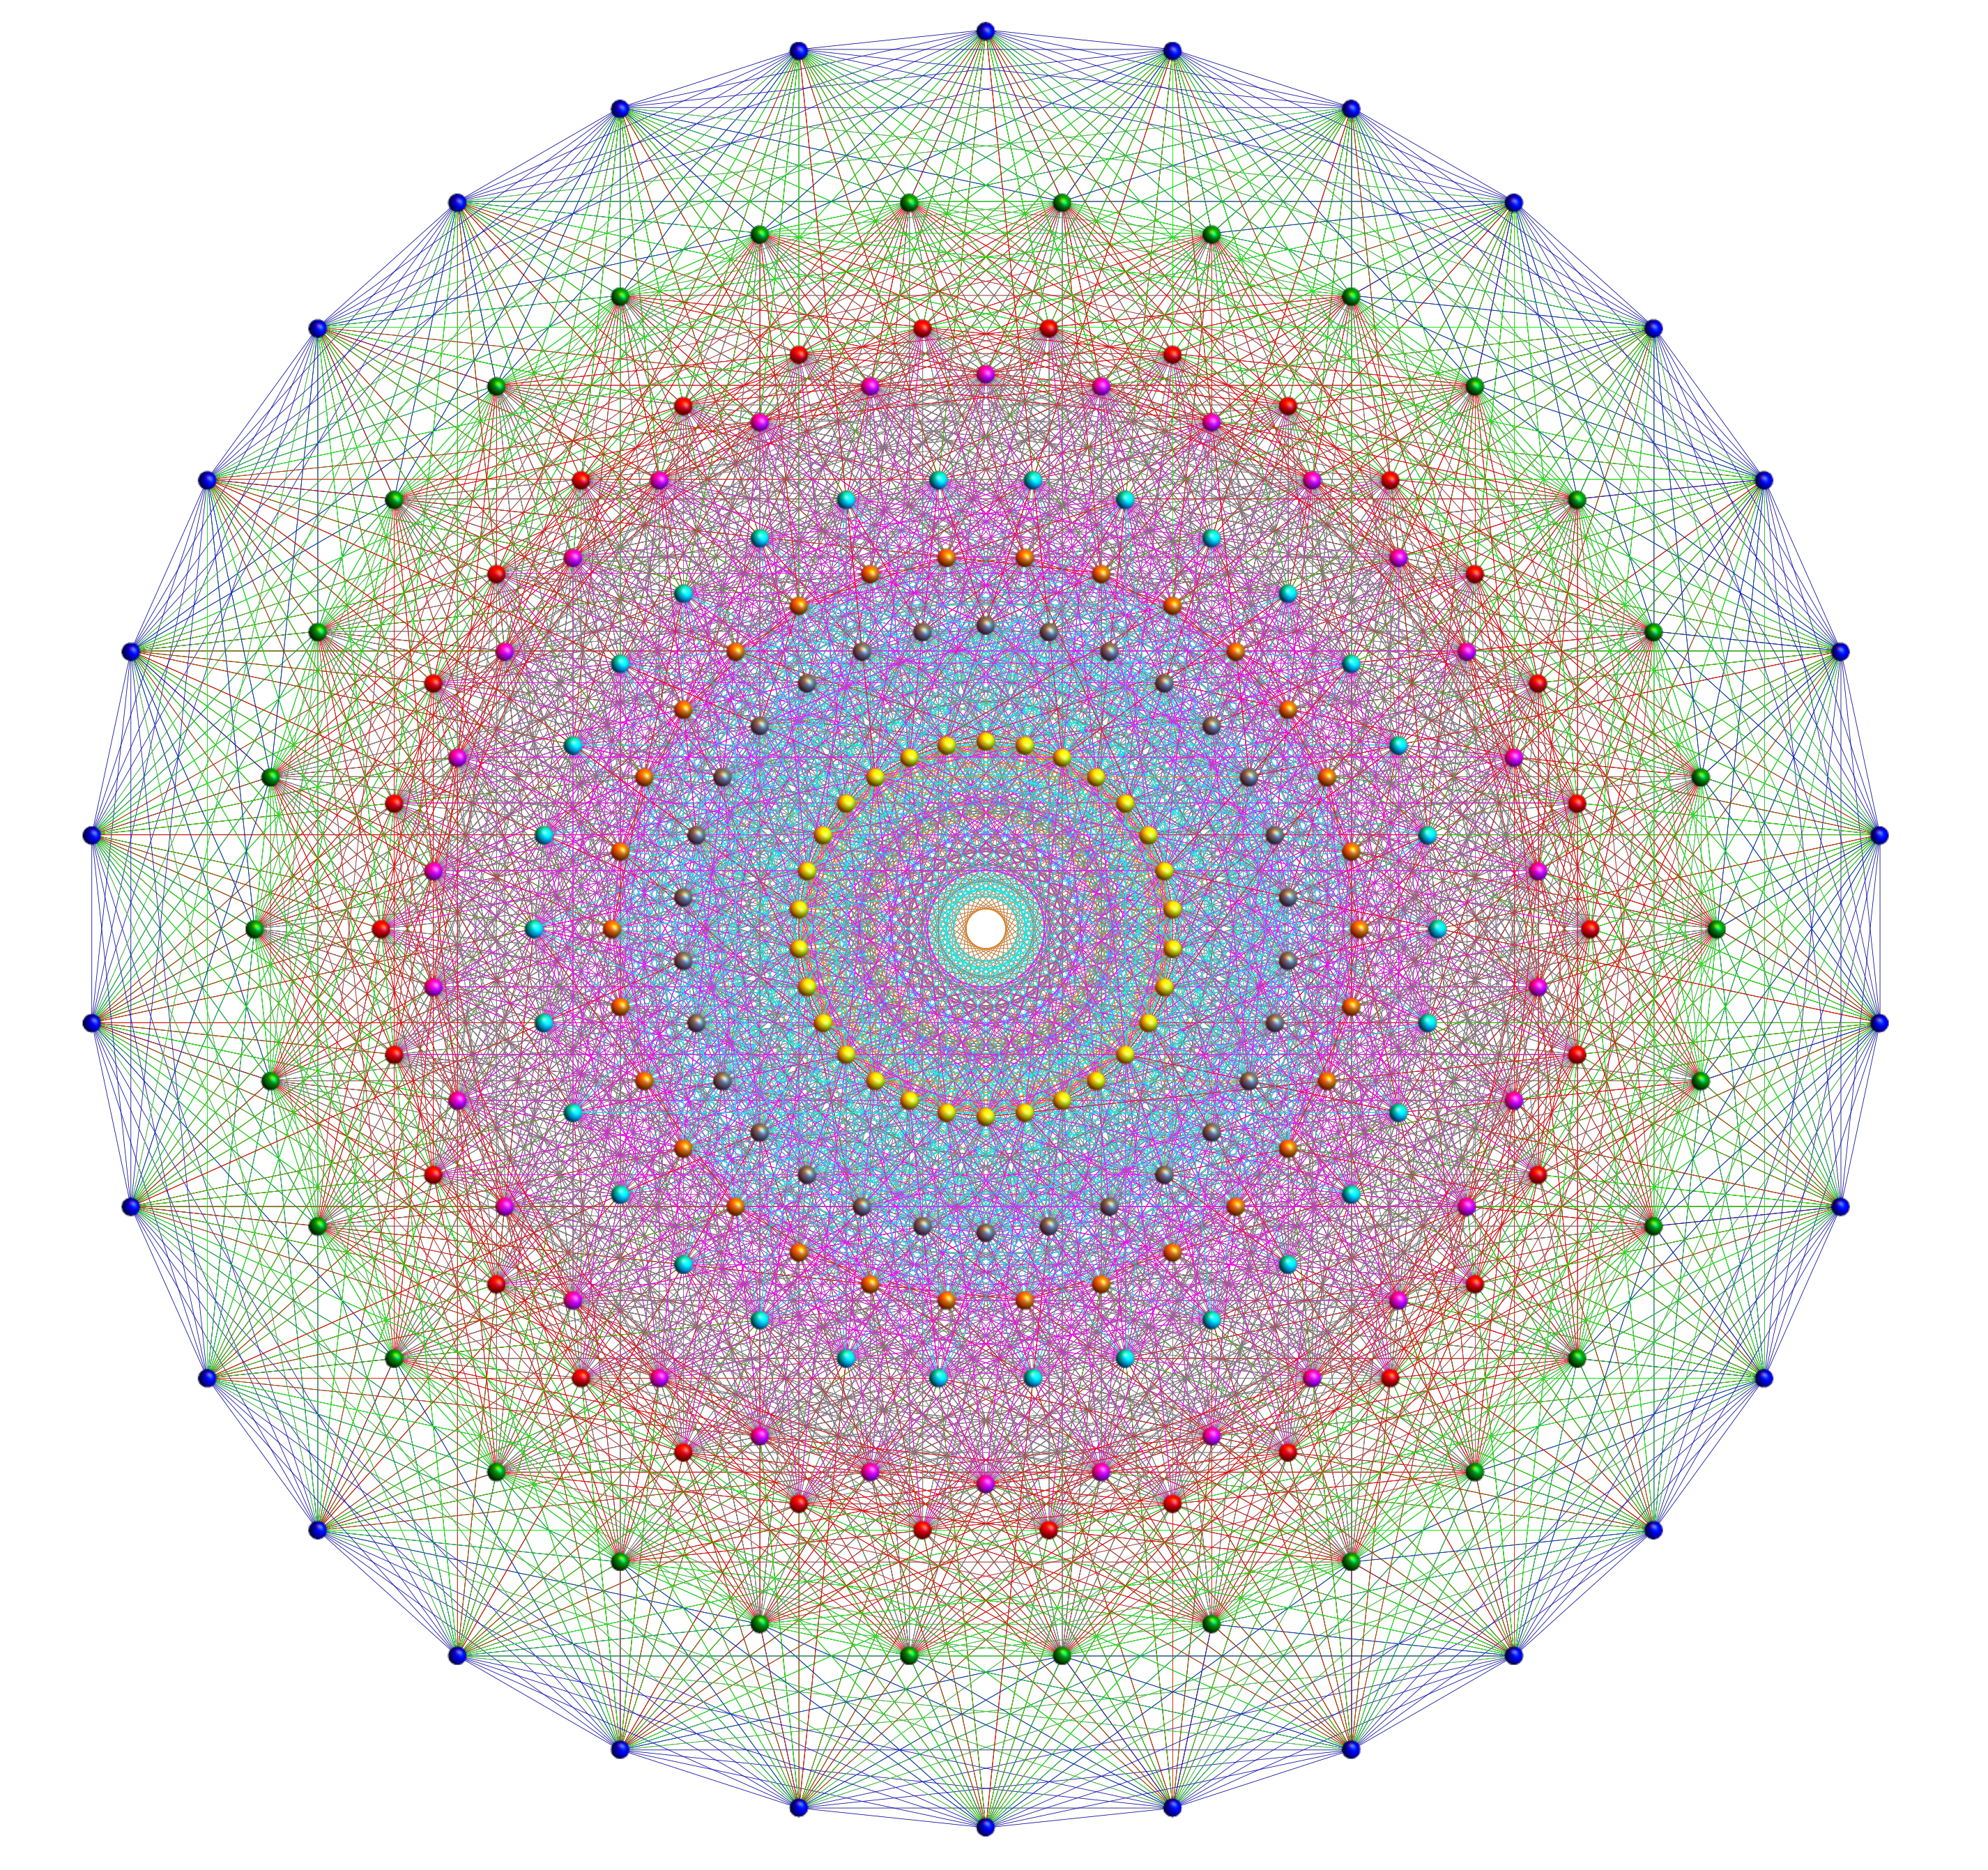
\includegraphics[width=1\columnwidth]{front.png}
\end{figure}
\newpage
\tableofcontents 
\newpage
\section{Gli interi}
\subsection{Propriet\`a di base}
Una propriet\`a dei numeri interi, che si prender\`a come assiomatica, \`e quella del \textit{buon ordinamento}: 
\begin{center}
	\textit{Ogni insieme non-vuoto di interi maggiori o uguali a $0$, ha un elemento minimo.}
\end{center}
Da questa deriva la seguente.
\begin{teorema}
	{Principio di induzione (prima forma)}{}
	Sia $A(n)$ un'affermazione valida per ogni intero $n\ge 1$ e si assume la possibilit\`a di dimostrare che:
	\begin{enumerate}[(1).]
		\item $A(1)$ \`e vera;
		\item $\forall n \ge  1$, se $A(n)$ \`e vera $\implies A(n+1)$ \`e vera.
	\end{enumerate}
	Allora, $\forall n \ge  1$, $A(n)$ \`e vera.
	\begin{proof}
		Sia $S $ l'insieme di interi per cui $A(n)$ \`e falsa. Si mostra che $S$ \`e l'insieme vuoto. 
		Assumendo per assurdo che $S\neq \varnothing\Rightarrow \exists n_0 \in S$, con $n_0$ minimo (esistente per il buon ordinamento), e, per assunzione, deve essere $n_0 \neq 1 \Rightarrow  n_0>1$. 
		Questo vuol dire che $n_0 -1$ non \`e in $S$ e, quindi, $A(n_0-1)$ \`e vera.

		Per la propriet\`a (2), per\`o, deve essere vera anche $A(n_0)$ perch\'e $n_0 = (n_0-1) + 1$, il che \`e assurdo e, pertanto, $S = \varnothing$.
	\end{proof}
\end{teorema}

\begin{obs}
	Nella dimostrazione sopra, si sarebbe potuto sostituire $1$ con $0$ e far partire il principio di induzione da $n=0$ piuttosto che da $n=1$ e non sarebbe cambiato nulla.
\end{obs}
\noindent Il principio di induzione pu\`o essere espresso in una forma alternativa, come segue.
\begin{teorema}
	{Principio di induzione (seconda forma)}{}
	Sia $A(n)$ affermazione vera $\forall n\ge 0$ e sia possibile mostrare che:
	\begin{enumerate}[(1').]
		\item $A(0)$ \`e vera;
		\item $\forall n > 0$, se $A(k)$ \`e vera $\forall 0\le k < n$, allora $A(n)$ \`e vera.
	\end{enumerate}
	Allora $A(n)$ \`e vera $\forall n\ge 0$.
	\begin{proof}
	Sia ancora $S$ l'insieme degli interi che non soddisfano $A(n)$. 
	Ancora per assurdo, si prende $S\neq \varnothing$, quindi deve esistere, per il buon ordinamento, un $n_0 \in S$ minimo.

	Per punto (1'), deve valere $n_0 \neq 0$ e, visto che $n_0$ \`e minimo, $\forall k$ intero tale che $0\le k< n_0$, $A(k)$ deve essere vera. 
	Per il punto (2'), per\`o, deve essere vera anche $A(n_0)$, arrivando nuovamente all'assurdo.
	\end{proof}
\end{teorema}
\noindent Un altro importante risultato del buon ordinamento \`e l'\textit{algoritmo di Euclide}.
\begin{teorema}
	{Algoritmo di Euclide}{}
	Siano $m,n$ interi, con $m>0$; allora esistono interi $q,r$, con $0\le r< m$, tali che
	\begin{equation}
		n = qm  + r
	\end{equation}
	Inoltre, gli interi $q,r$ sono univocamente determinati da tali condizioni.
	\begin{proof}
		Visto che l'insieme degli interi $q$ tali per cui $qm\le n$ \`e limitato superiormente per definizione, si pu\`o usare il buon ordinamento per affermare che esiste un elemento pi\`u grande tale che
		\[
		qm \le n < (q+1) m = q m + m
		\] 
		ossia $0\le n - qm < m$. Sia $r = n - qm$, per cui vale $0\le r < m$. Questo dimostra l'esistenza di $r,q$ come descritti.

		Per l'unicit\`a, si assume che valga contemporaneamente
		\[
		\begin{cases}
			n = q_1m + r_1&, \ 0\le r_1<m\\
			n = q_2m + r_2&, \ 0\le r_2<m\\
		\end{cases}
		\] 
		con $r_1 \neq r_2$. Sia, per esempio, $r_2> r_1$; allora, sottraendo le due, si ha $(q_1-q_2) m = r_2-r_1$. 
		Per\`o, si avrebbe $r_2-r_1> 0$, il che non \`e possibile perch\'e $q_1-q_2$ \`e un intero per cui $(q_1 - q_2)m > 0$, quindi si avrebbe $(q_1-q_2)m \ge m$.
		Pertanto, deve essere $r_1=r_2$, che fra l'altro implica $q_1m=q_2m$, per cui $q_1=q_2$.
	\end{proof}
\end{teorema}
\noindent Da questo teorema, si definisce $r$ come il \textit{resto della divisione di $n$ per $m$}.
\subsection{Massimo comune divisore}
Siano $n, d$ due interi diversi da $0$.
Si dice che $d$ \textit{divide} $n$ se esiste $q$ intero tale che $n = dq$; in questo caso, si scrive $d|n$.
Se $m,n$ sono interi non-nulli, per \textit{divisore comune} di $m$ e $n$ si intende un interno $d\neq 0$ tale che $d | m$ e $d | n$. 
Allora si ha la seguente definizione.
\begin{definizione}
	{Massimo comune divisore}{}
	Per massimo comune divisore di $m,n$ interi non nulli, si intende un intero $d>0$, divisore comune di $m$ e $n$, e tale che $\forall e $ intero positivo che divide $m$ e $n$, si ha anche $e|d$.
\end{definizione}
\noindent Chiaramente, il massimo comune divisore \`e univocamente determinato e si mostrer\`a che esiste sempre. 
Per farlo, si d\`a prima la seguente definizione.
\begin{definizione}
	{Ideale}{}
	Sia $J$ un sottoinsieme degli interi. Si dice che $J$ \`e un \textit{ideale} se:
	\begin{itemize}
		\item $0 \in J$;
		\item $m,n\in J\implies m+n \in J$
		\item se $m\in J$ e $n$ \`e un intero qualsiasi, allora $mn \in J$.
	\end{itemize}
\end{definizione}
\begin{esempio}
Siano $m_1, \ldots,m_r$ interi. Sia $J$ l'insieme di tutti gli interi che si scrivono come
\[
x_1m_1+\ldots+x_r m_r
\] 
con $x_1,\ldots,x_r$ interi. 
Allora \`e automaticamente verificato che $J$ \`e un ideale. Infatti
\begin{itemize}
	\item se $y_1,\ldots,y_r$ sono interi, allora
		\[
		\sum_{i=1}^{r} x_i m_i +  \sum_{j=1}^{r} y_j m_j = (x_1 + y_1) m_1 + \ldots + (x_r + y_r) m_r
		\] 
		che, quindi, appartiene a $J$;
	\item se $n$ \`e un intero, si ha
		\[
		n \sum_{i=1}^{r} x_i m_i = nx_1m_1 + \ldots+ nx_r m_r
		\] 
		che, quindi, appartiene a $J$;
	\item si pu\`o scrivere $0$ come $0m_1 + \ldots + 0m_r$, quindi anche $0 \in J$.
\end{itemize}
\end{esempio}
\noindent Dall'esempio precedente, si dice che $J$ \`e \textbf{generato} dagli interi $m_1,\ldots,m_r$ e che questi sono i suoi \textbf{generatori}.
Si nota che l'insieme $\left\{ 0 \right\} $ \`e esso stesso un ideale, chiamato \textbf{ideale nullo}. 
Inoltre, $\mathbb{Z}$ \`e detto \textbf{ideale unit\`a}.
Ora si pu\`o dimostrare il seguente.
\begin{teorema}
	{}{}
	Sia $J$ un ideale di $\mathbb{Z}$. Allora esiste un intero $d$ che \`e un generatore di $J$. Inoltre, se $J \neq \left\{ 0 \right\} $, allora $d$ \`e il pi\`u piccolo interno positivo in $J$.
	\begin{proof}
	Sia $J$ l'ideale nullo; allora $0$ \`e un suo generatore.
	Sia, ora, $J \neq \left\{ 0 \right\} $; se $n \in J$, allora $-n = (-1) n $ \`e anche in $J$, quindi $J$ contiene degli interi positivi.
	Si vuole dimostrare che $d$, definito come il pi\`u piccolo intero positivo, \`e un generatore.
	Per farlo, sia $n \in J$, con $n = dq + r, \ 0\le  r < d$; allora $r = n - dq \in J$ e, visto che vale $r < d$, segue che $r = 0$, quindi $n = dq$ e, allora, $d$ \`e un generatore.
	\end{proof}
\end{teorema}
\begin{teorema}
	{}{}
	Siano $m_1,m_2$ due interi positivi e sia $d$ un generatore positivo per l'ideale generato da $m_1,m_2$. Allora $d$ \`e il massimo comune divisore di $m_1,m_2$.
	\begin{proof}
		Per definizione, $m_1,m_2 \in J$\footnote{Questo \`e ovvio perch\'e $m_1 = 1m_1 + 0 m_2$ e $m_2  = 0 m_1 + 1 m_2$.}, quindi esiste un intero $q_1$ tale che $m_1=q_1 d$, per cui $d|
		m$.
		Analogamente $d|m_2$.
		Sia, poi, $e$ un intero non-nullo che divide sia $m_1$ che $m_2$ come $m_1 = h_1 e$ e $mm_2=h_2 e$, con interi $h_1,h_2$.
		Visto che $d$ \`e nell'ideale generato da $m_1,m_2$, esistono degli interi $s_1,s_2$ tali che $d = s_1m_1 + s_2m_2$, quindi
		\[
		d = s_1h_1e + s_2h_2e = (s_1h_1 + s_2h_2) e
		\] 
		Quindi $e $ divide $d$ e il teorema \`e dimostrato.
	\end{proof}
\end{teorema}
\begin{obs}
	La stessa esatta dimostrazione funziona per pi\`u di due interi, quindi se si considerassero $m_1,\ldots,m _r$ degli interi, con $d$ generatore positivo dell'ideale da loro generato, $d$ sarebbe anche il massimo comune divisore.
\end{obs}
\begin{definizione}
	{Interi relativamente primi}{}
	Siano $m_1,\ldots,m_r$ degli interi il cui massimo comune divisore \`e $1$. 
	Allora $m_1,\ldots,m_r$ si dicono \textit{relativamente primi} e, per questi, esistono interi $x_1,\ldots,x_r$ tali che
	\[
	x_1m_1   +\ldots + x_r m_r = 1
	\] 
	perch\'e $1$ appartiene all'ideale generato dagli $m_i$.
\end{definizione}
\subsection{Fattorizzazione unica}


\end{document}
